% !TeX root = main.tex
%************************************************************************
\section{Background}
\label{sec:background}
% List relevant work by others,
% or preliminary results you have achieved with a detailed and accurate
% explanation and interpretation.
% Include relevant photographs, figures or tables to illustrate the text.
% This section should frame the research questions that your subsequent research will address. 
%************************************************************************
This section gives some deeper background on the Web/App Framework, the editor I intend to build and what some common actions of users within the editor might be.
%************************************************************************
\subsection{Context of the Project and Problem Description} 
\label{sec:context}
%************************************************************************
In the following, I will only use the name ''app framework'' when referring to the meta-framework based on angular that can be deployed in Apps and as a Web-App.\\

To understand the usecases of the editor, I will first introduce you shortly to the app framework the editor should configure.
As described in the summary, the framework's build output is loaded from so called ''dynamic resources'', together with the configuration files, styling in form of css files, static images and other web contents.
At runtime, the framework reads the config files and renders the UI with a set of components. These components can be populated with data from datasources, change behaviour based on the ''context'', like device type,
query parameters in the URL or other external factors.

An simple example of an JSON configuration for a login view:

\begin{minted}[fontsize=\small]{json}
{
  "path": "login",
  "name": "login",
  "content": [
    {
      "type": "section",
      "class": "login-section",
      "content": [
        {
          "type": "html",
          "tag": "h1",
          "content": "LOGIN_TITLE"
        },
        {
          "type": "html",
          "tag": "p",
          "content": "LOGIN_IOS_TEXT",
          "condition": {
            "value": "$context.platform",
            "compareValue": "ios"
          }
        },
        {
          "type": "button",
          "message": "Login",
          "buttonClass": "button",
          "tap": {
            "type": "login"
          }
        }
      ]
    }
  ]
}
\end{minted}

Even with this basic example without any data sources or other complex dependencies, it is quite hard to undestand the mapping between configuration and generated UI, which leads to easily introduced errors.

Here are two screenshots of more complex UIs that can get configured with this framework:

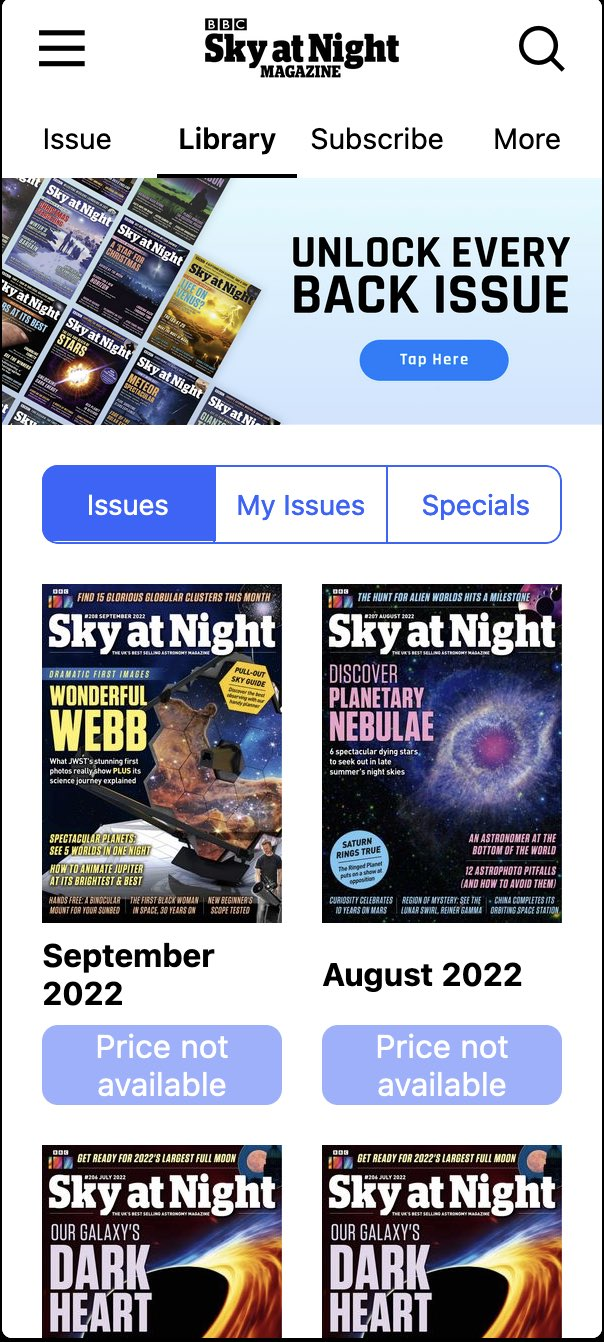
\includegraphics[height=15em]{pics/experience_screenshot_01.jpg}
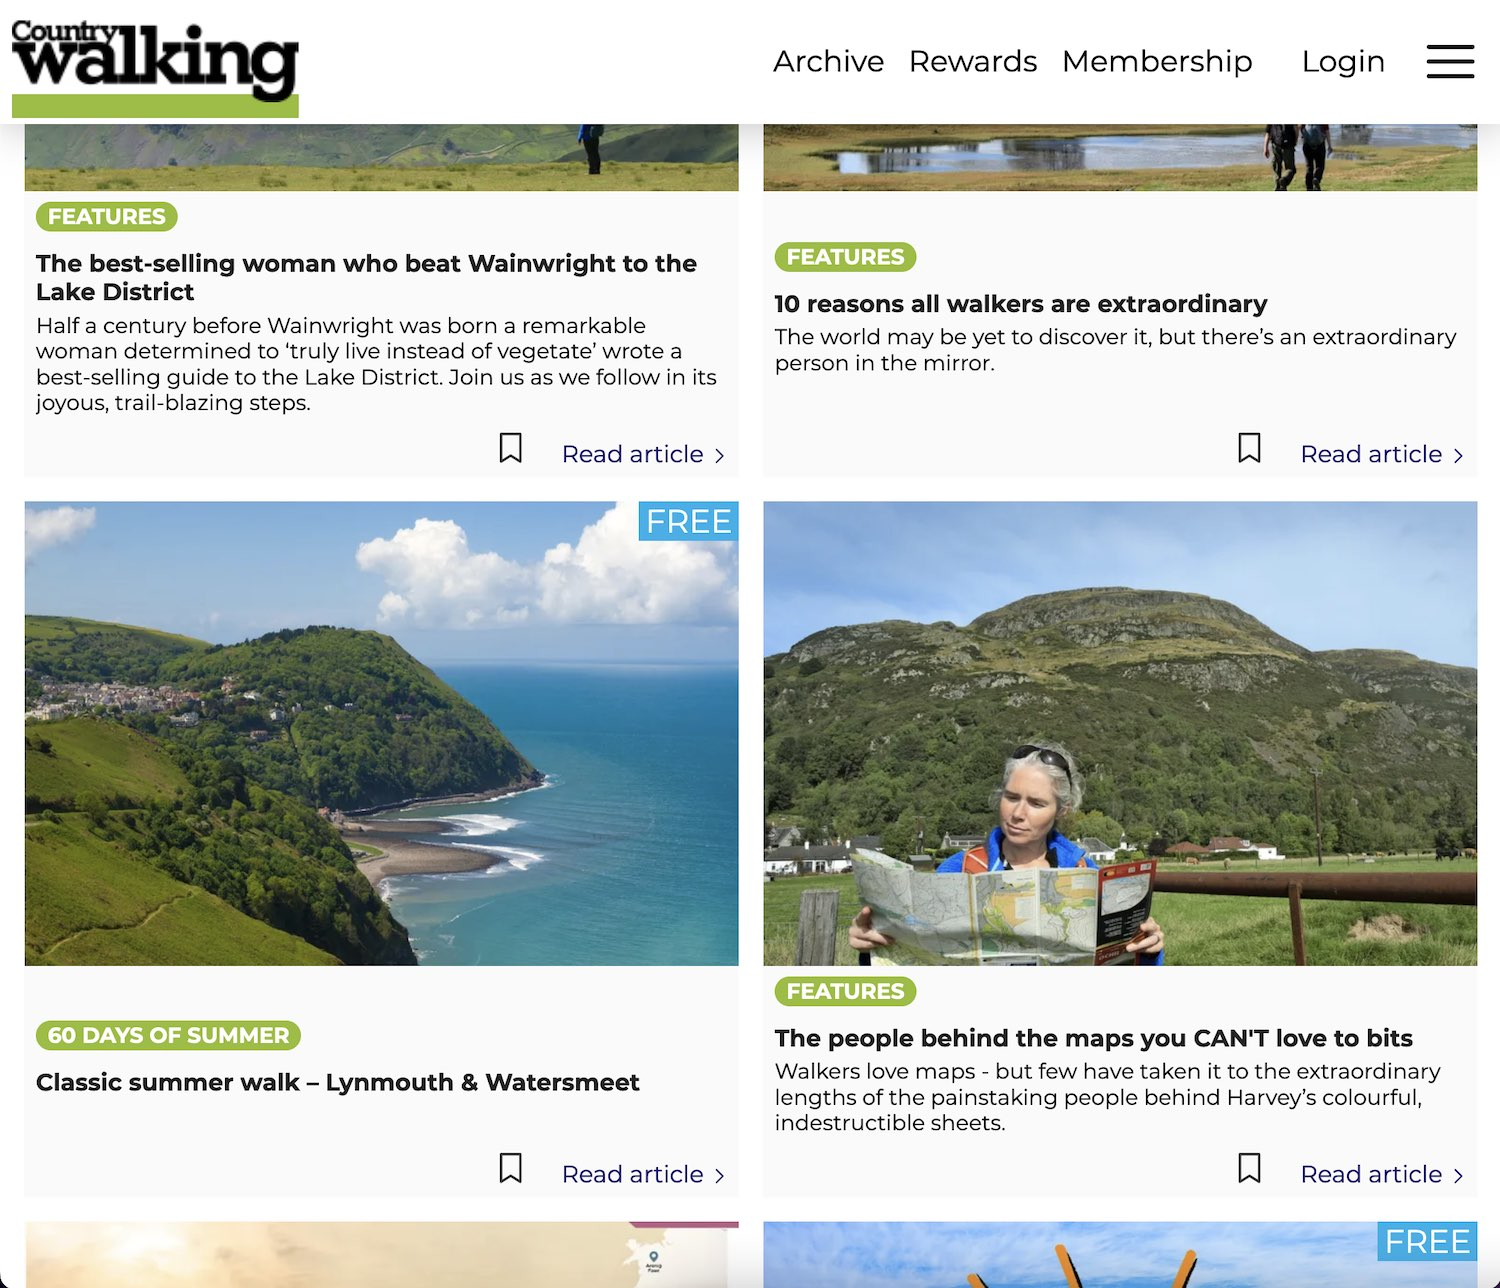
\includegraphics[height=15em]{pics/expeirence_screenshot_02.jpg}

The tasks performed depend a lot on the user; a admin from a publisher's company may just want to exchange an ad banner, rephrase some text or update a logo.
The Customer Success team at sprylab does more complex configurations like adapting exisitng apps for new customers by exchanging messages, colors, sometimes even adding complete views or adapt sections inside.
The framework developers use it for setting up new apps and features, confugirng complex filters for data sources and more.

Obviously, the easier the editor gets to use, the more the Customer Success and external users get enabled to do more changes on their own.
But it needs to be noted, that this system is constrained by the complexity of the schemas defining the UI configs. As this editor needs to work with the exisitng schematas, there is a limit on how easy it will be to configure apps, but the goal is to push this boundary further than current workflows allow.

%************************************************************************
\subsection{Related Work}
\label{sec:relatedwork}
%************************************************************************
This section consists of a literature review to situate your thesis in the scientific context. Which academic articles exist in your problem area, and how are they related to your work? When placing your thesis in the context of others, you need to consider other work, which uses a similar methodology or articles, who try to answer similar research questions.

The related work can be split into two (or even three) parts.

\subsubsection{JSON Editor - generative UI}

\begin{itemize}
	\item \href{https://f1000research.com/articles/11-475}{Adamant: a JSON schema-based metadata editor for research data management workflows}
	\item \href{https://json-schema.org/understanding-json-schema/UnderstandingJSONSchema.pdf}{Understanding JSON Schema}
	\item \href{https://www.researchgate.net/publication/220728636_Interactive_model_driven_graphical_user_interface_generation}{Interactive model driven graphical user interface generation }
	\item \href{https://www.sciencedirect.com/science/article/pii/S2352711018300505}{JSON-GUI}
\end{itemize}

Example Implementations which should get evaluated or taken as reference
\begin{itemize}
	\item \url{https://github.com/json-editor/json-editor}
	\item \url{https://jsonforms.io/}
\end{itemize}



\subsubsection{Sources for HCI methods and UI design}

\begin{itemize}
	\item \href{https://www.diva-portal.org/smash/get/diva2:215020/FULLTEXT01.pdf }{Methods and Qualities of a Good User Interface Design}
	\item \href{}{Book: Lern human computer interaction, Christopher Reid Becker}
	\item \href{}{Book: Interaction Design: Beyond Human-Computer Interaction }
	\item \href{https://citeseerx.ist.psu.edu/viewdoc/download?doi=10.1.1.75.2615&rep=rep1&type=pdf}{INTEGRATING HUMAN-COMPUTER INTERACTION DEVELOPMENT INTO THE SYSTEMS DEVELOPMENT LIFE CYCLE: A METHODOLOGY}
	\item \href{https://wso2.com/library/articles/2019/04/brownfield-integration-why-its-important-for-modernizing-your-enterprise/}{Brownfield Integration: Why It's Important For Modernizing Your Enterprise}
\end{itemize}

%************************************************************************
\subsection{Research Questions}
\label{subsec:question}
% Based on your overarching goal and the reviewed research, specify your research question.
%************************************************************************
How does an editor for dynamic resources for users with different levels of expertise look like and how can it be conceptualized and implemented within the constraints of an exisiting ecosystem?


Other questions that fit into the thesis topic: \\
\begin{itemize}
  \item What pain points can be solved by existing libraries and tools, which require new development or enhancement?
  \item What challenges arise when applying HCI methods in a brownfield development process and how can they be dealt with?
  \item How can we improve the user experience for people with no knowledge about the system, while also giving powerusers the amount of flexability they need?
\end{itemize}
